% Sample LaTex for CSC 482/582
% I have cut out sections of the writing which
% were not illustrative of important formatting.
%
\documentclass[12pt]{article}
%
\usepackage[export]{adjustbox}
\usepackage{multirow}
\usepackage{amsmath}
\usepackage{algorithm}
\usepackage{array}
\newcolumntype{L}{>{\centering\arraybackslash}m{3cm}}


\usepackage[noend]{algpseudocode}

% This nextcommand lets you put in .eps files as figures.
%
\usepackage{epsfig}

% This next command gives 1.5 spacing which I would
% like in your submissions so there is room to
% give feedback.

\renewcommand{\baselinestretch}{1.5}
% These mean a common numbering scheme is given for
% theorems, conjectures, corollaries and lemmas.
% The numbering depend on which section they are in.
\newtheorem{theorem}{Theorem}[section]
\newtheorem{conjecture}[theorem]{Conjecture}
\newtheorem{corollary}[theorem]{Corollary}
\newtheorem{lemma}[theorem]{Lemma}
\newcommand{\wbeginproof}{ \noindent {\em Proof. }}
\newcommand{\wendproof}{\bigskip}
\begin{document}
\title{ Generating Polyhedral Molecules from Planar Embeddings of 3-Regular Graphs}
\author{Wendy Myrvold \\ University of Victoria 
\and David Mitchell  \\ University of Victoria 
}
\maketitle
\section{Introduction}

An \textit{undirected graph} G consists of a set of vertices V(G) and a set of edges E(G) where each edge corresponds to an unordered pair of vertices \cite{BM}. The sets V(G) = \{0, 1, 2, 3, 4, 5, 6, 7\} and E(G) = \{(0,1), (0,2), (0,3), (1,2), (1,3), (2,4), (3,5),  (4,6), (4,7), (5,6), (5,7), (6,7)\} represent the undirected graph G shown in Figure \ref{Figure1}. A graph is \textit{connected} if for every partition of V(G) into two non-empty sets A and B there is an edge containing a vertex from A and a vertex from B \cite{BM}. 

\begin{figure}[H]
    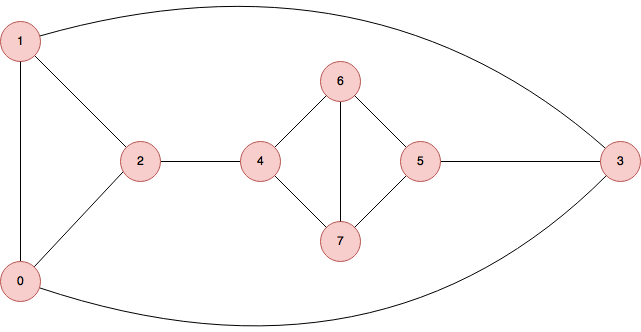
\includegraphics[scale=.4, center]{Figure1}
    \caption{Planar embedding of undirected graph G}
    \label{Figure1}
\end{figure}

The vertices of the graphs we will generate represent either carbon atoms or nitrogen atoms. The edges represent bonds between atoms. While these graphs contain no self-loops in which a vertex is connected to itself by an edge, multiple edges between vertices are allowed. For example, the undirected graph H represented by V(H) = \{0, 1, 2, 3\} and E(H) = \{(0,1), (0,1), (0,2), (1,3), (2,3), (2,3)\} shown in Figure \ref{Figure2} contains multiple edges.

\begin{figure}[H]
    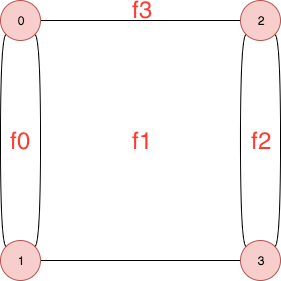
\includegraphics[scale=.4, center]{Figure2}
    \caption{Planar embedding of graph H with multiple edges}
    \label{Figure2}
\end{figure}


The \textit{degree} of a vertex $v$ is the number of edges incident to $v$ \cite{BM}. If a graph is 3-regular, then every vertex has degree three and the graph is called \textit{cubic}. The graphs shown in Figures \ref{Figure1} and \ref{Figure2} are examples of cubic graphs.

A graph which can be drawn in the plane so that no two edges intersect except at the vertices is called \textit{planar} and a representation in the plane is a \textit{planar embedding} \cite{WM1}. A graph can be embedded on the plane if and only if it is also embeddable on the sphere. A planar embedding partitions the plane into faces. The set of faces F(H) of graph H in Figure \ref{Figure2} is \{$f_0, f_1, f_2, f_3$\} where $f_0, f_1$ and $f_2$ are bounded faces and $f_3$ is the external face.

If S is a subset of the vertices V(G) such that every vertex is either in S or is adjacent to a vertex in S then S is a called a \textit{dominating set} \cite{BM}. As well, if S is a subset of the vertices V(G) such that no vertex in S is adjacent to another vertex in S then S is called an \textit{independent set} \cite{BM}. The set S = \{2,5\} of graph G in Figure \ref{Figure1} constitutes a dominating set which is also an independent set.

For S $\subseteq$ V, the subgraph H induced by S has V(H) = S and E(H) = \{(u,v): (u,v) $\in$ E(G), u $\in$ S and v $\in$ S\} \cite{BM}. The graph in Figure \ref{Figure3} is an induced subgraph of G on the vertices S = \{0,4,5,6,7\}. 

\begin{figure}[H]
    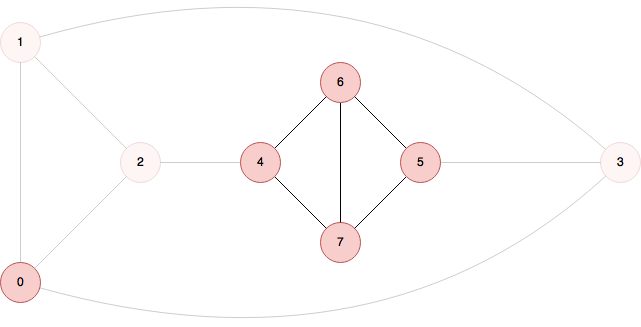
\includegraphics[scale=.4,center]{Figure3}
    \caption{Subgraph of G induced by S}
    \label{Figure3}
\end{figure}


A \textit{matching} (which is also referred to as an independent set of edges) is a set of edges in which no two edges are incident to the same vertex \cite{BM}. In a perfect matching, every vertex of the graph is incident to an edge in the matching. The set of edges \{(0,1), (2,4), (3,5), (6,7)\} in Figure \ref{Figure4} is a perfect matching. 

\begin{figure}[H]
    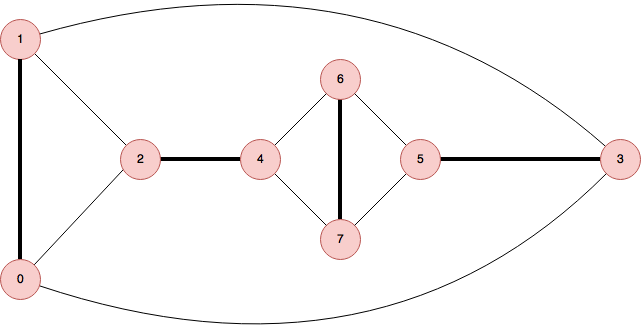
\includegraphics[scale=.4,center]{Figure4}
    \caption{A perfect matching}
    \label{Figure4}
\end{figure}

The objective of our research is to discover a graph-theoretical solution to a problem pertaining to the generation of new polyhedral molecules \cite{PF}. Specifically, we wish to generate polyhedral molecules that are composed of carbon, nitrogen and hydrogen atoms and have the steric requirements that bonds between nitrogen atoms are avoided and each carbon atoms has a bond to exactly one other carbon atom. The resulting molecules are restricted to the molecular formula $N_{4q}(CH)_{6q}$ where q is a positive integer. Each nitrogen atom is bonded to three carbon atoms and each carbon atom is bonded to two nitrogen atoms, one carbon atom and one hydrogen atom, although the hydrogen vertices of the CH pairs are suppressed in our representation. Our aim is to generate planar embeddings which fit these requirements by modelling each molecule as a cubic graph composed of vertices labelled N or C. The graph of Figure \ref{Figure5} is an example of a solution.

\begin{figure}[H]
    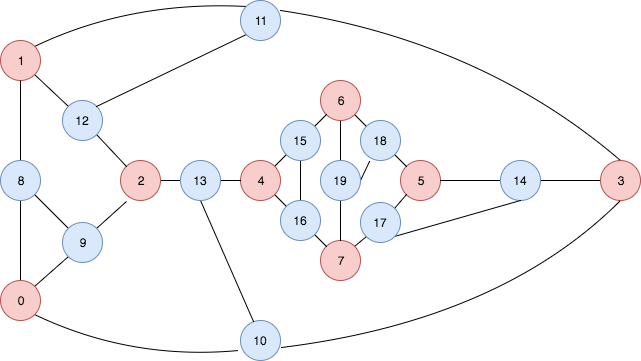
\includegraphics[scale=.4,center]{Figure5}
    \caption{A solution of molecular formula $N_{8}(CH)_{12}$. N vertices are red and C vertices are blue.}
    \label{Figure5}
\end{figure}


\section{Data Structures for Graph Embeddings}

An \textit{adjacency list} is a collection of n lists, one for each vertex $v_i$ where $0 \leq i \leq n-1$, in which each entry in the list is a vertex to which $v_i$ is adjacent. A \textit{rotation system} is an adjacency list which describes a circular ordering of the graph's edges around each vertex. A rotation system for a planar embedding of a graph lists the neighbouring vertices in clockwise order. For this application, an array is used to store the contents of each list in the rotation system. 

If a graph has multiple edges, the edges are not uniquely defined by the vertices they are incident upon. Edge numbers are assigned to each edge $e$ to identify them.

Figure 6 is a representation of the embedding of G in Figure 1 using a rotation system.
\begin{figure}[H]
{\footnotesize
\begin{center}
\begin{tabular}{|c|c|} 
\hline
$v_i$ & neighbour vertex (edge number) \\
\hline

0 & 1 (0), 2 (1), 3 (2) \\
1 & 0 (0), 3 (3), 2 (4) \\
2 & 0 (1), 1 (4), 4 (5) \\
3 & 0 (2), 5 (6), 1 (3) \\
4 & 2 (5), 6 (7), 7 (8) \\
5 & 3 (6), 7 (9), 6 (10) \\
6 & 4 (7), 5 (10), 7 (11) \\
7 & 4 (8), 6 (11), 5 (9) \\

\hline
\end{tabular}
\end{center}
}
\caption{A representation of Figure \ref{Figure1} using a rotation system}
\label{Figure6}
\end{figure}

Given a rotation system, Algorithm 1 can be used to \textit{walk the faces} of an embedding, where walking a face means to traverse the boundary of the face \cite{WM3}.

\begin{algorithm}[H]
\caption{Face walking algorithm for a planar embedding}\label{euclid}
\begin{algorithmic}[1]
\scriptsize
\Procedure{WalkFaces}{G}
    \State \# G is a graph object which contains a rotation system denoted adj\_list that is an array of vertices
    \State \# v.return\_neighbour(G,j) returns the vertex at position j in v's array of neighbours
    \State \# v.next\_pos\_after\_edge(e) returns 1 + position of e mod v.num\_nbrs in v's array of edges \\

    \For{i in 0..G.num\_vertices-1}
        \State v $\gets$ G.adj\_list[i]
        \For {j in 0..v.num\_nbrs - 1}
            \State v.nbrs[j].visited $\gets$ False
        \EndFor
    \EndFor
    \For{i in 0..G.num\_vertices-1}
        \State v $\gets$ G.adj\_list[i]
        \For {j in 0..v.num\_nbrs - 1}
            \If {v.nbrs[j].visited == False}
                \State first\_edge = v.edges[j]
                \State curr\_edge = first\_edge
                \State curr\_v = v.return\_neighbour(G,j)
                \State first $\gets$ True

\algstore{myalg}
\end{algorithmic}
\end{algorithm}
 
\begin{algorithm}[H]
\begin{algorithmic}[1]
\algrestore{myalg}
\scriptsize    
                \While {curr\_edge != first\_edge or first}
                    \State first $\gets$ False
                    \State pos = curr\_v.next\_pos\_after\_edge(curr\_edge)
                    \State curr\_v.nbrs[pos].visited $\gets$ True
                    \State curr\_edge = curr\_v.edges[pos]
                    \State curr\_v = curr\_v.return\_neighbour(G,pos)
                \EndWhile    
            \EndIf
        \EndFor
    \EndFor
\EndProcedure
\end{algorithmic}
\end{algorithm}

\section{Isomorphism Testing of Embeddings}

The \textit{canonical form} for our graph embeddings is the lexicographically smallest labelling of the vertices and their neighbours in the rotation system using clockwise breadth first search. If two rotation systems have the same canonical form, they are isomorphic to one another \cite{WM4}. An \textit{isomorphism} of a rotation system representing an embedding is a bijection from a rotation system G to a rotation system H such that any two vertices which are adjacent in G are adjacent in H and any ordering of vertices in G are ordered identically in H or reversed. 

Algorithm 2 is an algorithm for clockwise breadth first search \cite{WM2}.

\begin{algorithm}[H]
\caption{Clockwise breadth first search}\label{euclid}
\begin{algorithmic}[1]
\scriptsize
\Procedure{CW\_BFS}{G, root, first\_child}
    \State \# v.return\_nbr\_pos(nbr) returns the position of nbr in v's neighbour array 
    \State \# parent\_pos[i] maintains the position of the parent of the ith vertex in v's neighbour array \\
    \State parent\_pos, queue $\gets$ [ ]
    \State queue.push(root)
    \State parent\_pos[root] $\gets$ root.return\_nbr\_pos(first\_child)
    \While {!queue.empty?}
        \State v $\gets$ q.shift
        \For {i in 0..v.num\_nbrs-1}
            \State nbr\_v $\gets$ v.return\_nbr(parent\_pos[v]+i $\bmod$ 3)
            \If {parent\_pos[nbr\_v] = nil}
                \State queue.push(nbr\_v)
                \State parent\_pos[nbr\_v] $\gets$ nbr\_v.return\_nbr\_pos(vertex)
            \EndIf
        \EndFor
    \EndWhile           
\EndProcedure
\end{algorithmic}
\end{algorithm}


\section{Finding Solutions}
One approach to discovering molecules with the desired characteristics would be to factor all planar embeddings of the 3-regular graphs into sets of C and N vertices. However, for the majority of graphs this factorization is not possible. Further, there are too many embeddings to feasibly generate and check each of them beyond graphs with a smaller set of vertices. The number of cubic connected graphs with 2n nodes is given in Table \ref{table1}.

{\scriptsize
\begin{center}
\begin{table} [H]
\resizebox{\textwidth}{!}{%
\begin{tabular}{ |c|c|c|c| } 
\hline
n & \# of cubic graphs with 2*n vertices & n & \# of cubic graphs with 2*n vertices  \\
\hline
0	&	1 & 10	&	510,489\\
1	&	0 & 11 & 7,319,447\\
2	&	1 & 12 & 117,940,535\\
3	&	2 & 13 & 2,094,480,864\\
4	&	5 & 14 & 40,497,138,011\\
5	&	19 & 15 & 845,480,228,069\\
6	&	85 & 16 & 18,941,522,184,590\\
7	&	509 & 17 & 453,090,162,062,723\\
8	&	4,060 & 18 & 11,523,392,072,541,432 \\
9	&	41,301 & 19 & 310,467,244,165,539,782 \\
\hline
\end{tabular}}
\caption{OEIS A002851 Number of unlabeled trivalent (or cubic) connected graphs with 2n nodes. \cite{OEIS} }
\label{table1}
\end{table}
\end{center}}

A different approach is suggested by observing characteristics of embeddings which are solutions. First, the C-C edges of the molecule are a perfect matching on the subgraph induced by the C vertices. Second, the set of N vertices are a dominating set of the solution. Third, the set of N vertices are also an independent set.

If the C-C edges of any solution is removed, the result is a planar embedding in which each C vertex has degree two and the edges from any C vertex are incident to two distinct N vertices. In Figure \ref{Figure7}, the C-C edges of the solution in Figure \ref{Figure5} are removed. 

\begin{figure}[H]
    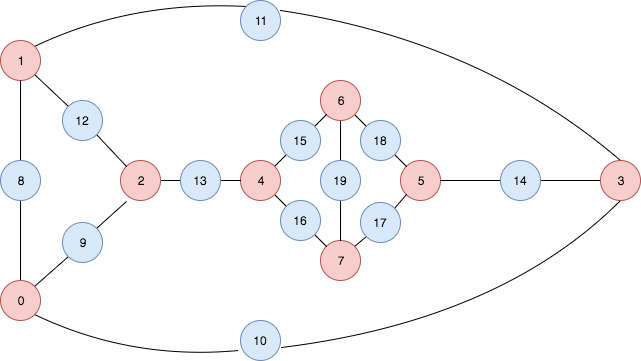
\includegraphics[scale=.4,center]{Figure7}
    \caption{The solution of Figure \ref{Figure5} with C-C edges removed}
    \label{Figure7}
\end{figure}

Further, if we perform a series reduction on a series N-C-N to N-N for every series N-C-N in the embedding, the result is a smaller, 3-regular planar embedding.

\begin{figure}[H]
    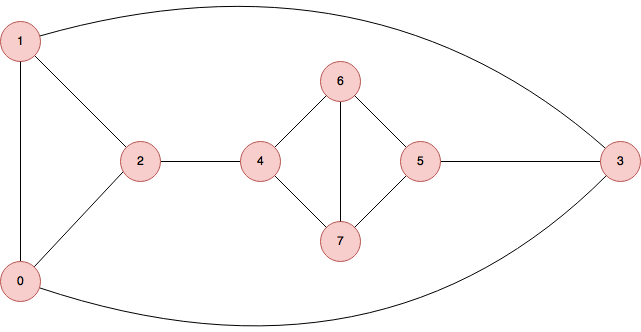
\includegraphics[scale=.4,center]{Figure1}
    \caption{Underlying 3-regular planar embedding}
    \label{Figure8}
\end{figure}

Our observations propose a constructive algorithm for finding molecules which are solutions. We begin with a planar embedding of a smaller cubic graph for which each vertex is labelled N. We subdivide each edge with a vertex labelled C. Finally, we add edges next to vertices of degree two while maintaining planarity in all ways until the embedding is 3-regular. The constructed 3-regular embedding is a solution.

\begin{figure}[H]
    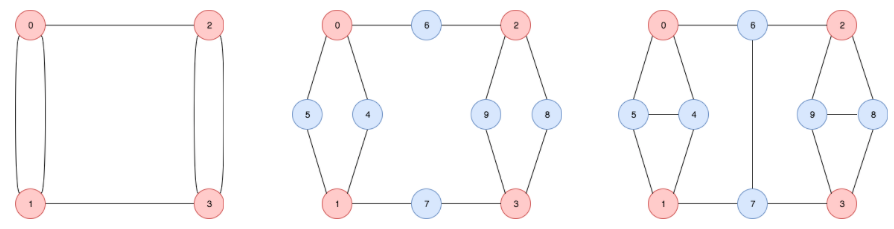
\includegraphics[scale=.4,center]{Figure9}
    \caption{Constructive algorithm for finding solutions}
    \label{Figure9}
\end{figure}

\section{Generating Algorithm - Connected Case}
We begin with the rotation system of a planar embedding of a connected 3-regular graph in which every vertex is labelled N. Each edge of the embedding is then bisected by a C vertex numbered the current number of vertices in the graph.

\begin{algorithm} [H]
\caption{N-N edge bisection}\label{euclid}
\begin{algorithmic}[1]
\scriptsize
\Procedure{Bisect}{G}
    \State \#v.new(i,`C') creates a new vertex numbered i with label 'C'
    \State \#v.add\_nbr(u) adds the vertex number of u to the first empty position in v's neighbour array
    \State \#v.replace\_nbr(u,w) replaces the vertex number of u with w in v's neighbour array \\
    \For{i in 0..G.num\_vertices-1}
        \State v $\gets$ G.adj\_list[i]
        \For{j in 0..v.num\_nbrs-1}
            \State nbr\_v $\gets$ v.return\_nbr(G,j)
            \If{nbr\_v.label == `N'}
                \State edge\_num $\gets$ v.edges[j]
                \State new\_v $\gets$ v.new(G.num\_vertices,`C')
                \State new\_v.add\_nbr(v)
                \State new\_v.add\_nbr(nbr\_v)
                \State G.add\_v(new\_v)
                \State v.replace\_nbr(nbr\_v,new\_v,j)
                \State pos $\gets$ nbr\_v.return\_edge\_pos(edge\_num)
                \State nbr\_v.replace\_nbr(v,new\_v,pos)
            \EndIf
        \EndFor
    \EndFor
\EndProcedure

\end{algorithmic}
\end{algorithm}

Chords are then added to each C vertex in all ways maintaining planarity using a recursive backtracking algorithm as follows. Beginning with the lowest numbered vertex labelled `C', $v$, a list of the vertices to which a chord can be added is generated by walking the faces v is incident to and adding any degree two vertices $u_i$ such that the number of vertices before bisection $\leq$ i and i $<$ number of vertices after bisection. A chord is added from v to the first $u_i$ on the list and the algorithm is called on the following C vertex. When every vertex on the graph has degree three, the rotation system is printed. When the algorithm returns, the chord is removed and a chord is added to the next vertex $u_i$ on the list. When the list is exhausted, the algorithm returns.

\begin{algorithm}
\caption{Generate graphs by adding chords in all ways and maintaining planarity}\label{euclid}
\begin{algorithmic}[1]
\scriptsize
\Procedure{add\_chords}{G, level}
    \State \# level is an int indicating the number of the vertex to which chords are being added to
    \State \# G.get\_candidates(v) walks the faces of v and returns an array of candidate objects
    \State \# a candidate contains a vertex to add a chord to and its position in the rotation system

    \If{level == G.num\_vertices}
        \State G.output\_graph
        \State return
    \EndIf
    
    v = G.adj\_list[level]
    
    \If{v.num\_nbrs $<$ 3}
        \State candidates = G.get\_candidates(v) 
        \For{Each candidate c}
            \State G.connect\_vertices(v,c)
            \State add\_chords(G,level+1)
            \State G.disconnect\_vertices(v,c)
        \EndFor
    \Else
        \State add\_chords(level+1)
    \EndIf
\EndProcedure

\end{algorithmic}
\end{algorithm}

\section{Canonical Form}

If two graphs output by the graph generation algorithm are isomorphic to one another, they are considered duplicates. A set of unique solutions is found by listing the canonical form of each solution and removing duplicates. The canonical form for each graph is found by traversing the embedding and the flip of an embedding using clockwise breadth first search on each vertex and its neighbours. In the flip of an embedding the neighbours are listed in reverse order. The vertices and its edges are then renamed in the order in which they are discovered in the breadth first search. 

\begin{algorithm}[H]
\caption{Output the canonical form of the embedding} \label{euclid}
\begin{algorithmic}[1]
\scriptsize
\Procedure{find\_cf}{G}
    \State \# CW\_BFS is a modified version of clockwise breadth first search that returns an embedding with vertices and edges renumbered by the index in which they are discovered
    \State \# compare\_cfs(min\_cf,cf) returns -1 if min\_cf is lexicographically smaller than cf, 0 if equal and otherwise 1
    \State \# flip(G) returns an embedding of G in which each vertex's neighbours are listed in reverse order \\

    \State min\_cf
    \State F $\gets$ flip(G)
    \For{d in 0..1}
        \If{d == 0}
            \State g $\gets$ G
        \Else
            \State g $\gets$ F
        \EndIf
        \For{i in 0..g.num\_vertices-1}
            \State v $\gets$ g.adj\_list[i]
            \For{j in 0..v.num\_nbrs-1}
                \State cf $\gets$ CW\_BFS(g,v,j)    
                \If{min\_cf == nil}
                    \State min\_cf $\gets$ cf
                \Else 
                    \If {compare\_cfs(min\_cf,cf) == -1}
                        \State min\_cf $\gets$ cf
                    \EndIf
                \EndIf
            \EndFor
        \EndFor
    \EndFor
\EndProcedure

\end{algorithmic}
\end{algorithm}

\section{Computational Results}

Solutions were generated for the connected case of 3-regular planar embeddings without multiple edges for graphs with up to 12 vertices. To obtain these results, the planar 3-regular embeddings that were used in the construction were generated by plantri by Gunnar Brinkmann (University of Ghent) and Brendan McKay (Australian National University).

The canonical form of each solution using clockwise breadth first search was calculated and duplicate solutions were removed. The results are stated in Table \ref{table2}.

\begin{table}[H]
\begin{center}
\begin{tabular}{ |L|L|L|L| } 
\hline
\# vertices in underlying graph & \# vertices in bisected graph & \# of solutions generated & \# of solutions generated less duplicates \\
\hline
4 & 10 & 8 & 1 \\
8 & 20 & 790 & 121 \\
12 & 30 & 420,078 & 172,821 \\
\hline
\end{tabular}
\end{center}
\caption{Results of generating solutions in the connected case with no multiple edges}
\label{table2}
\end{table}

\section{Future Work}

Solutions for the cases of 3-regular planar embeddings with multiple edges and multiple components have not been generated. The algorithm we have described can be applied to the cases of multiple edges to arrive at a complete solution. However, in the cases of a graph with multiple components, the face walking algorithm must be revised to traverse the external edges of all disconnected components for every vertex incident to the external face. The constructive algorithm for the disconnected case is demonstrated in Figure \ref{Figure10}.    

\begin{figure}[H]
    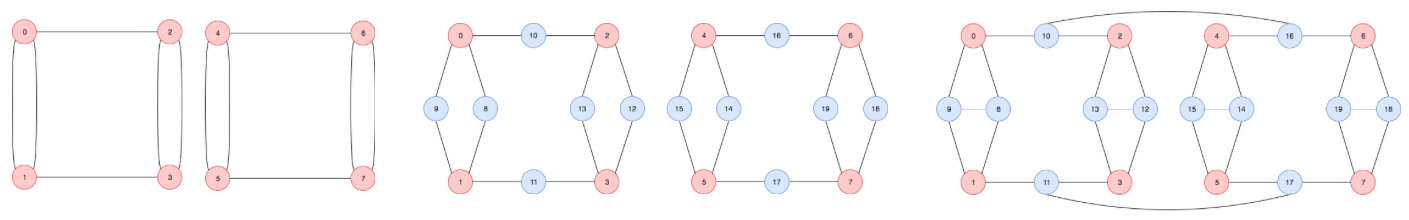
\includegraphics[scale=.4,center]{Figure10}
    \caption{Constructive algorithm for finding solutions in the disconnected case}
    \label{Figure10}
\end{figure}

\bibliographystyle{plain}
\bibliography{tan}
\end{document}
